\chapter{20-Time, Revolutions}

\section{Question 1}

In this sprint, we wanted to add 3 main new features. The first was the ability to add a high score. The idea behind this was that the scores could be kept and seen again, and that there would be a high score screen to show what the top scores for the game were. The second feature was the ability to have options, so that for example the music could be turned off by the player, if they do not like it. The final thing we wanted to add to our game, was a boss. The boss has to have the ability to shoot the player. To make this boss harder to kill we gave the boss a few lives. Now when you have completed all the normal levels, the boss level appears, and when you kill the boss you win the game.

\section{Question 2}

\subsection{Introduction}

For the boss, two new classes had to be add, 'FinalEnemy' and 'BubbleEnemy', both these classes are related to other classes. \\\\
For adding the high score two classes have been added. These are the NameInputController and HighscoreEntryController classes. 

\subsection{Responsibility Driven Design} 

\subsubsection{FinalEnemy}
\textit{Responsibility:} \\
The final enemy has to be able to move from the top to the bottom of the screen, and it has to be able to shoot a BubbleEnemy. When the player hits the final enemy with it's bubble, he has to lose a life. \\ \\
\textit{Collaborations:} \\
FinalEnemy collaborates with Observable to be able to send updates to Observer classes. It also collaborates with  the SpriteBase, to get the x and y, and with both the Bubble extensions, to fire bubbles and to be shot by bubbles.

\subsubsection{BubbleEnemy}
\textit{Responsibility:} \\
The BubbleEmey's are shot by the FinalEnemy, these bubbles have the ability to move through walls. When one of these bubbles hits the player, the player has to die. \\ \\
\textit{Collaborations:} \\
BubbleEnemy collaborates with Observable to be able to send updates to Observer classes. It also collaborates with  the SpriteBase, to get the x and y, with the FinalEnemy to be shot by, and with the Player to kill.

\subsubsection{High score}
\textit{Responsibility:} \\
The StartController asks the name(s) of the player(s) via the NameInputController. The highscores are build up of HighscoreEntryControllers, which gets and sets the scores in Settings. \\ \\
\textit{Collaborations:} \\
StartController collaborates with NameInput and HighscoreEntryController to manage custom player names for the high scores. HighscoreEntryController collaborates with Settings to save and retrieve the high scores so they are saved even after the game is stopped.

\subsubsection{Options}
\textit{Responsibility:} \\
The preferences screen request the preferences to update the UI. \\
The different objects request properties with a certain key, Settings retrieves the property. All objects can also set properties via Settings. Settings communicates with the Java Properties class, which relies on a HashMap, responsible for the key-value mapping. \\ \\
\textit{Collaborations:} \\
Settings collaborates with Properties to store and retrieve the values for given keys.

\subsection{UML}

\subsubsection{High score}

The following UML is for the High Score feature.
\\\\
\includegraphics[width=100mm]{HighscoreUML.png}

\subsubsection{Options}
The following UML is for the Options feature.
\\\\
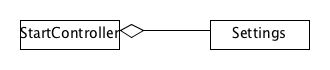
\includegraphics[width=100mm]{Options_UML.png}

\subsubsection{Final Boss}

The following UML is the UML for the Boss feature.
\\\\
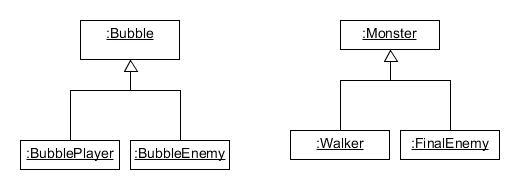
\includegraphics[width=100mm]{FinalEnemyUml.png}



